\chapter{System Overview}
\label{chap:overview}
At a cloud cluster node, each instance of a guest operating system runs on a virtual machine, accessing virtual hard disks 
represented as virtual disk image files in the host operating system.
For VM snapshot backup, file-level semantics are normally not provided.
Snapshot operations take place at the virtual device driver level, which
means no fine-grained file system metadata can be used to determine the changed data. 
Backup systems have been developed to use content fingerprints to identify duplicate
content~\cite{venti02,Rhea2008}.  
As discussed earlier, collocating a backup service on the existing
cloud cluster avoids the extra cost to acquire a dedicated backup facility
and reduces the network bandwidth consumption in transferring the
raw data for backup. 
% Figure~\ref{fig:collocated} illustrates the cluster architecture where
% each physical machine runs a backup service and a distributed file system (DFS)~\cite{googlefs03,hdfs10}
% serves a backup store  for the snapshots.
Figure~\ref{fig:collocated} illustrates a converged IaaS cloud architecture
where each commodity server hosts a number of virtual machines and storage of these servers
is clustered using a distributed file system~\cite{googlefs03,hdfs10}.
Each physical machine hosts multiple virtual machines.  Every virtual machine
runs its own guest operating system and accesses virtual hard disks
stored as image files maintained by the operating system running on the
physical host.

\begin{figure}[htb]
    \centering
    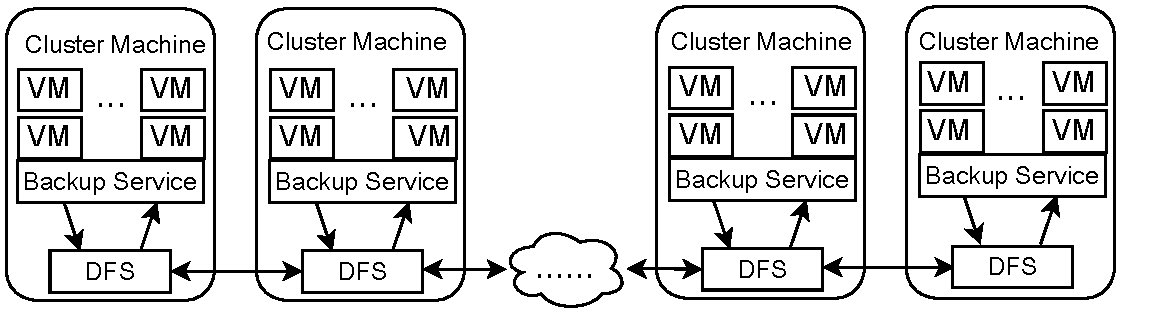
\includegraphics[width=5in]{images/colocated-arch}
    \caption{VM snapshot backup running on a converged cloud cluster.}
    \label{fig:collocated}
\end{figure}

\section{Snapshot Service Overview}
\label{overview:ss}
We will briefly introduce the abstraction of our storage architecture here 
and discuss the implementation details in chapter~\ref{chap:data}.
Our architecture is built on the Aliyun platform which provides the largest public VM cloud in China 
based on Xen~\cite{Xen2003}. A typical VM cluster in our cloud environment
consists of from hundreds to thousands of physical machines, each of which can
host tens of VMs.

A GFS-like distributed file system holds the responsibility of managing physical disk storage
in the cloud. All data needed for VM services, which include runtime VM disk images and snapshot backup data,
reside in this distributed file system.
During the VM creation, a user chooses her flavor of OS distribution and the cloud system 
copies the corresponding pre-configured base VM image to her VM as the OS disk, 
and an empty data disk is created and mounted onto her VM as well. 
All these virtual disks are represented as virtual machine image files in our
underline runtime VM storage system. The runtime I/O between virtual machine and its virtual
disks is tunneled by the virtual device driver (called TapDisk\cite{Warfield2005} at Xen). To avoid network latency and congestion, 
our distributed file system place the primary replica of VM's 
image files at physical machine of VM instance.
During snapshot backup, concurrent disk write is logged 
to ensure a consistent snapshot version is captured. 

Figure~\ref{fig:arch} shows the architecture view of our snapshot service
at each node. The snapshot broker provides the functional interface for snapshot backup, access, and deletion.
The inner-VM  deduplication is conducted by the broker to access meta data in the snapshot data store
and we discuss this in details in Section~\ref{sect:innerVM}.
The cross-VM deduplication is conducted by the broker to access 
a popular data set (PDS) (will discuss in Section~\ref{sect:crossVM},
whose block hash index is stored in a distributed memory cache. 

\begin{figure}[htbp]
  \centering
  %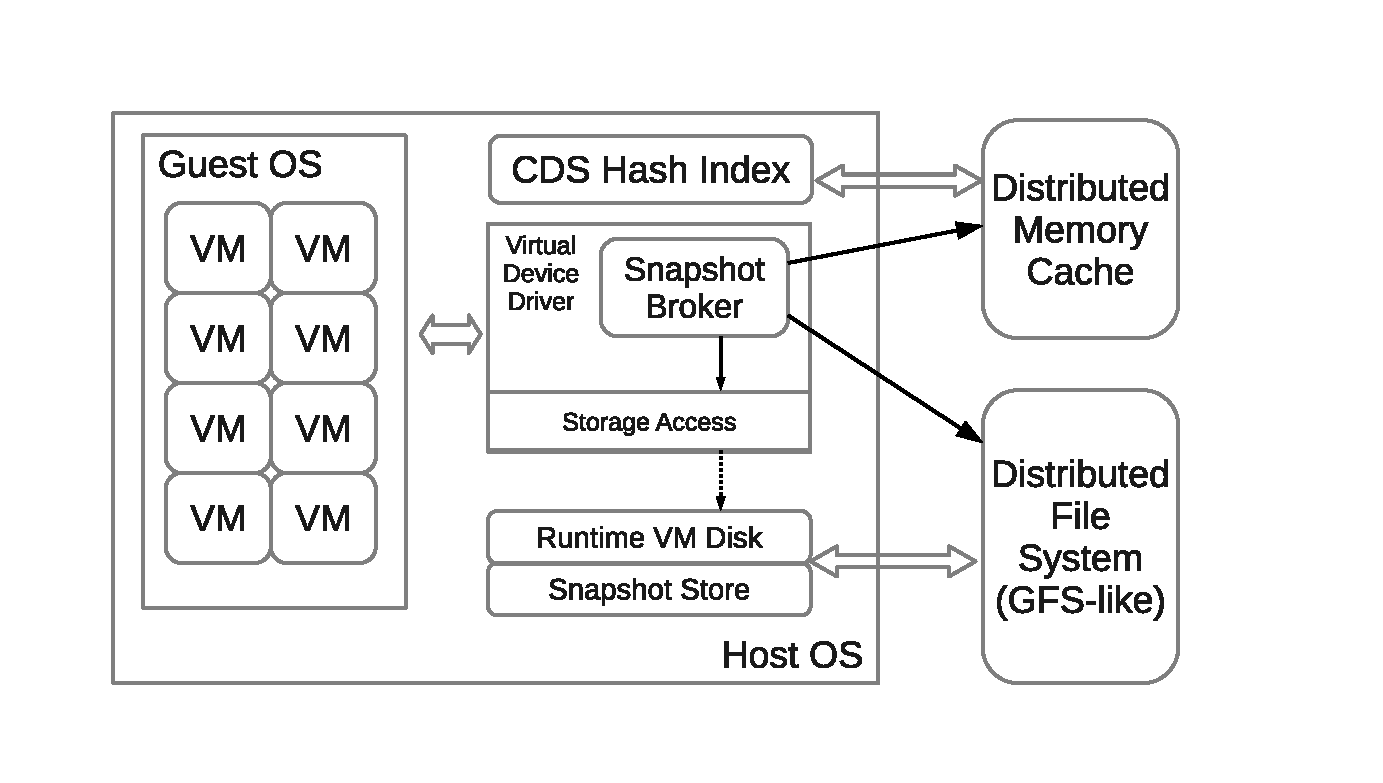
\epsfig{file=images/arch.eps, height=2in, width=2.66in}
  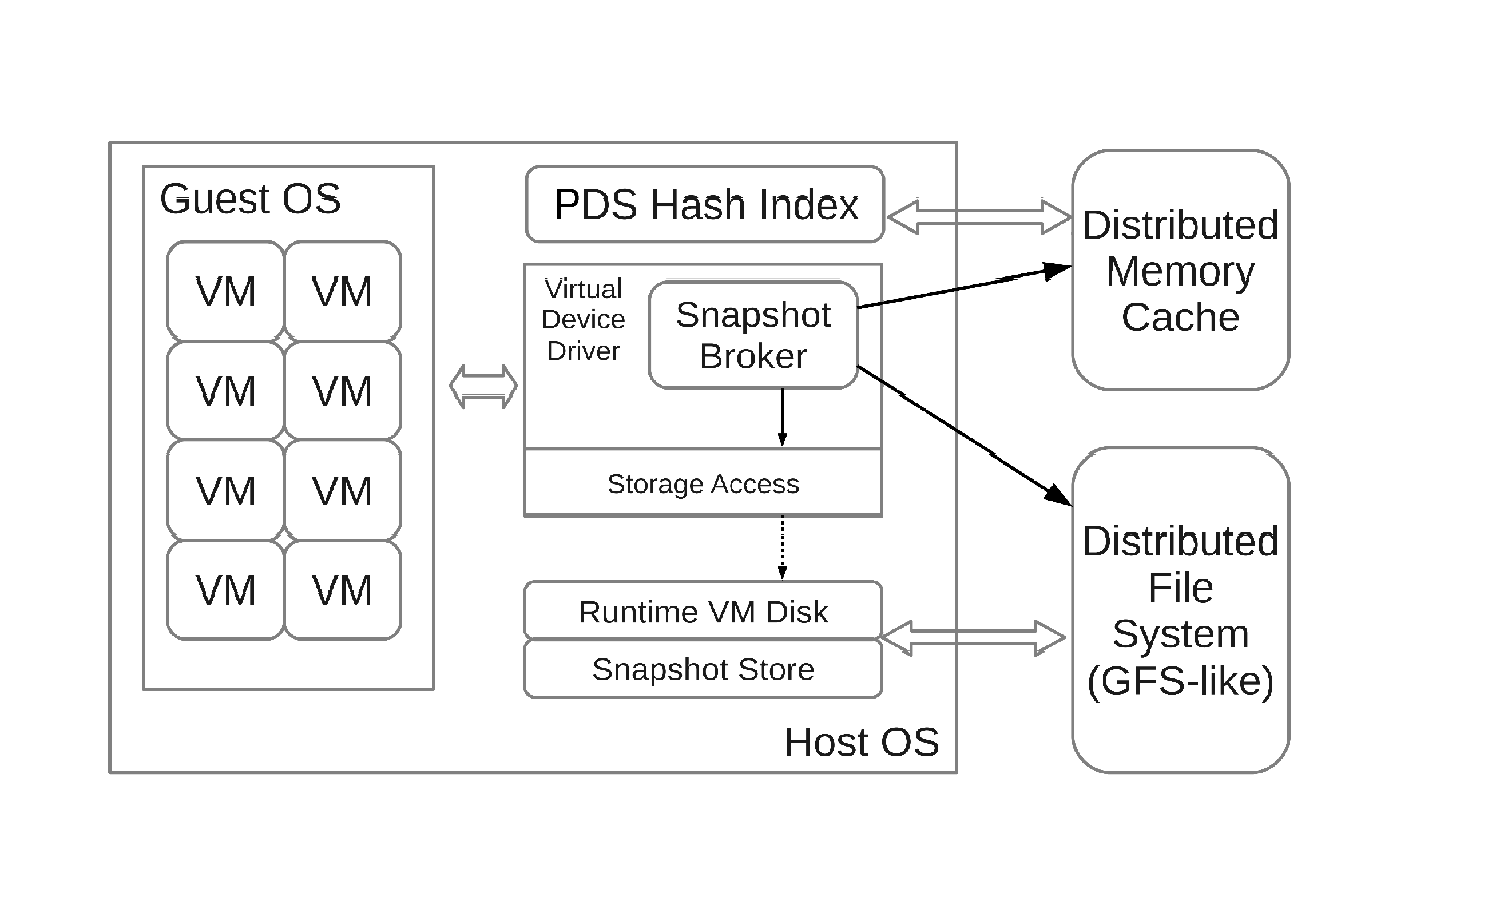
\includegraphics[width=5in]{images/arch1.pdf}
  \caption{Snapshot backup architecture abstraction}
  \label{fig:arch}
\end{figure}

The snapshot store 
supports data access operations such as \emph{Get}, \emph{Append} and \emph{Delete}.
Other operations include data block traverse and resource usage report.
The snapshot data does not need to be
co-located with VM instances, and in fact they can even live in a different cluster to improve the 
data reliability: when one cluster is not available, we are still able to restore its VMs from another cluster which
holds its snapshot data. 
%to reduce the impact to our users.
%Get interface accepts a piece of data, write it to the underline data file, and return
%a reference to the caller. This reference then can be used in the put interface to
%retrive or delete the data, thus the caller of put interface must preserve the
%data reference for future use. 
%In addition to above standand data access operations, the snapshot service also supports
%\emph{scan} and \emph{quota} methods. Scan allows us to traverse all the data blocks of each VM
%in the snapshot store, and quota is used to acknowledge user how much space he
%has actually used.

Under the hood of snapshot store, it organizes and operates snapshot data 
in the distributed file system. We let each virtual disk has its own snapshot store, 
and no data is shared between
any two snapshot stores, thus achieve great fault isolation. For those selected popular data
that shared by many VM snapshot stores, we could easily increase its availability by having more replications.
%Since all the underline data structures is append only,
%upon a delete request, the corresponding data will only be marked rather than being deleted.
%A compaction will take place when deleted data has accumulated to a certain threshold, thus 
%reclaiming the disk space .


%The detail design and implementation of our distributed file system and various 
%storage subsystems would be too complicated to be intorduced here, and also beyond
%the scope of this paper. In the remaining section we will brief the model and interface of 
%our snapshot storage.


\section{VM Snapshot Metadata Hierarchy}
\label{overview:meta}

\begin{figure}[htbp]
  \centering
  %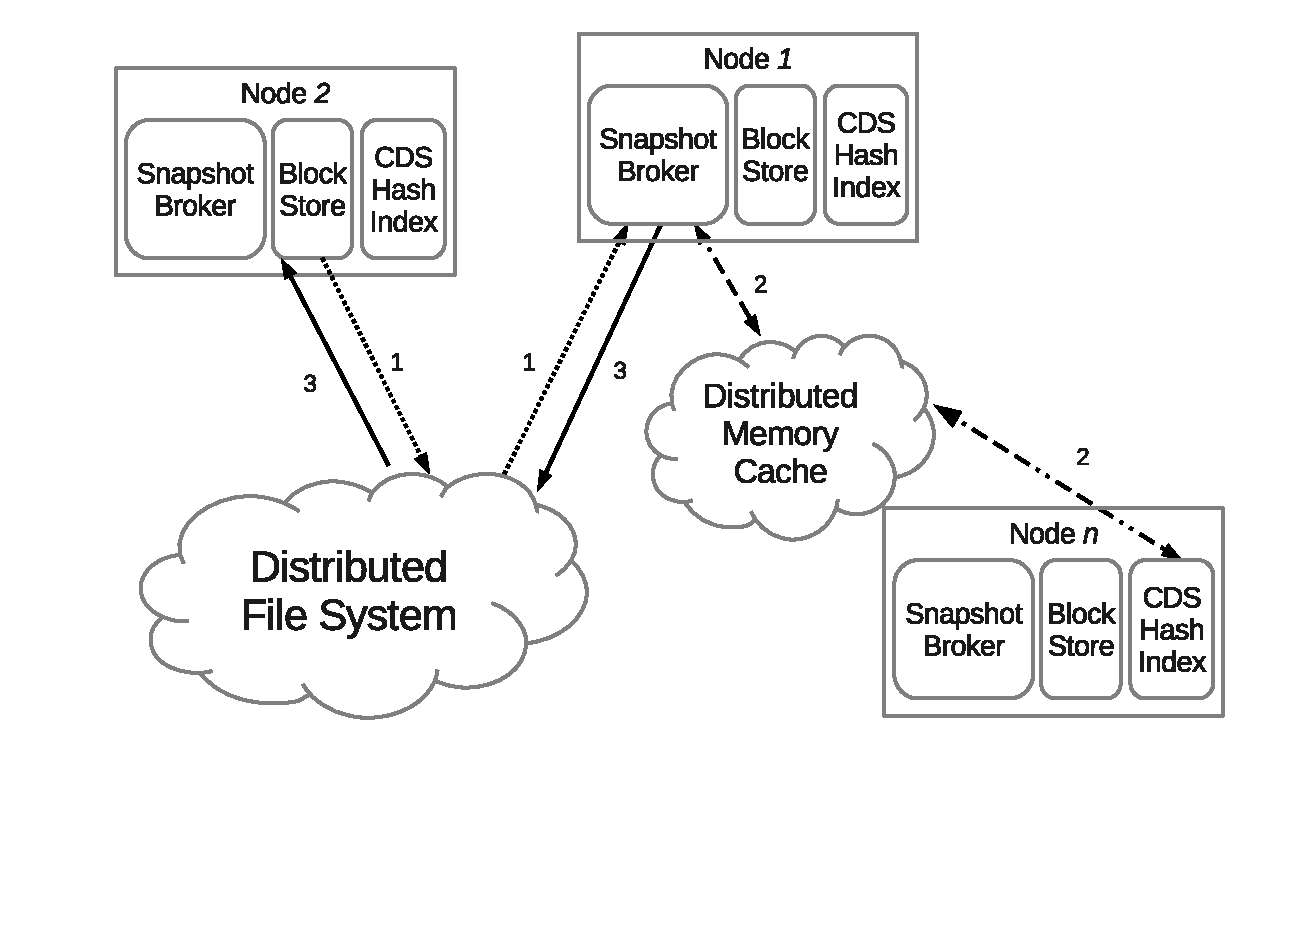
\epsfig{file=images/dedup_process.eps, height=2in, width=2.66in}
  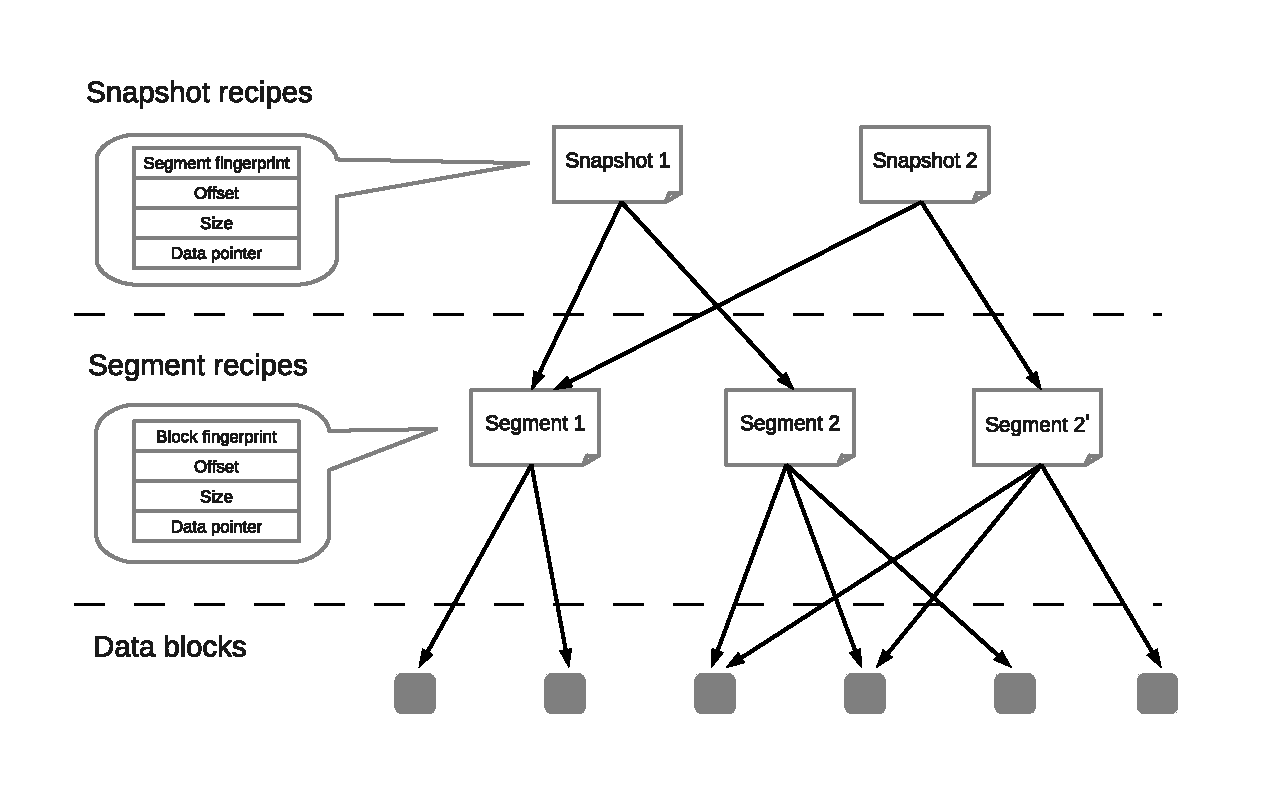
\includegraphics[width=5in]{images/snapshot_representation.pdf}
  \caption{An example of snapshot representation.}
  \label{fig:snapshot}
\end{figure}

The representation of each snapshot in the backup
storage has a two-level index structure in the form of a
hierarchical directed acyclic graph as shown in Figure~\ref{fig:snapshot}.
A VM image is divided into a set of segments and each
segment contains content blocks of variable-size, partitioned using the standard chunking technique with 4KB
as the average block size. The snapshot metadata contains a list of segments and other meta data information.
Segment metadata contains its content block fingerprints
and reference pointers. If a segment is not changed from
one snapshot to another, indicated by a dirty bit embedded in the virtual disk driver, its segment metadata contains a reference pointer to an earlier segment. For a
dirty segment, if one of its blocks is duplicate to another
block in the system, the block metadata contains a reference pointer to the earlier block.

